\chapter[High-Throughput Calculation and Machine Learning Predictions]{High-Throughput Calculation and Machine Learning Predictions} \label{c:result-1} 

In this chapter, we describe the generation of hypothetical organic spacers and the subsequent prediction of their properties using a combined high-throughput DFT approach and machine learning techniques. Section \ref{section:section4-1} outlines the systematic expansion of the organic spacer library through molecular morphing operations. Section \ref{section:section4-2} presents general physical insights derived from high-throughput DFT calculations. Sections \ref{section:section4-3} and \ref{section:section4-4} discuss the selection and evaluation of machine learning models, highlighting their predictive performance and their role in extracting structure-property relationships.


\section{Molecular generation for chemical space expansion}\label{section:section4-1}

\subsection{Morphing operation}

\begin{figure}[htbp]
    \centering
    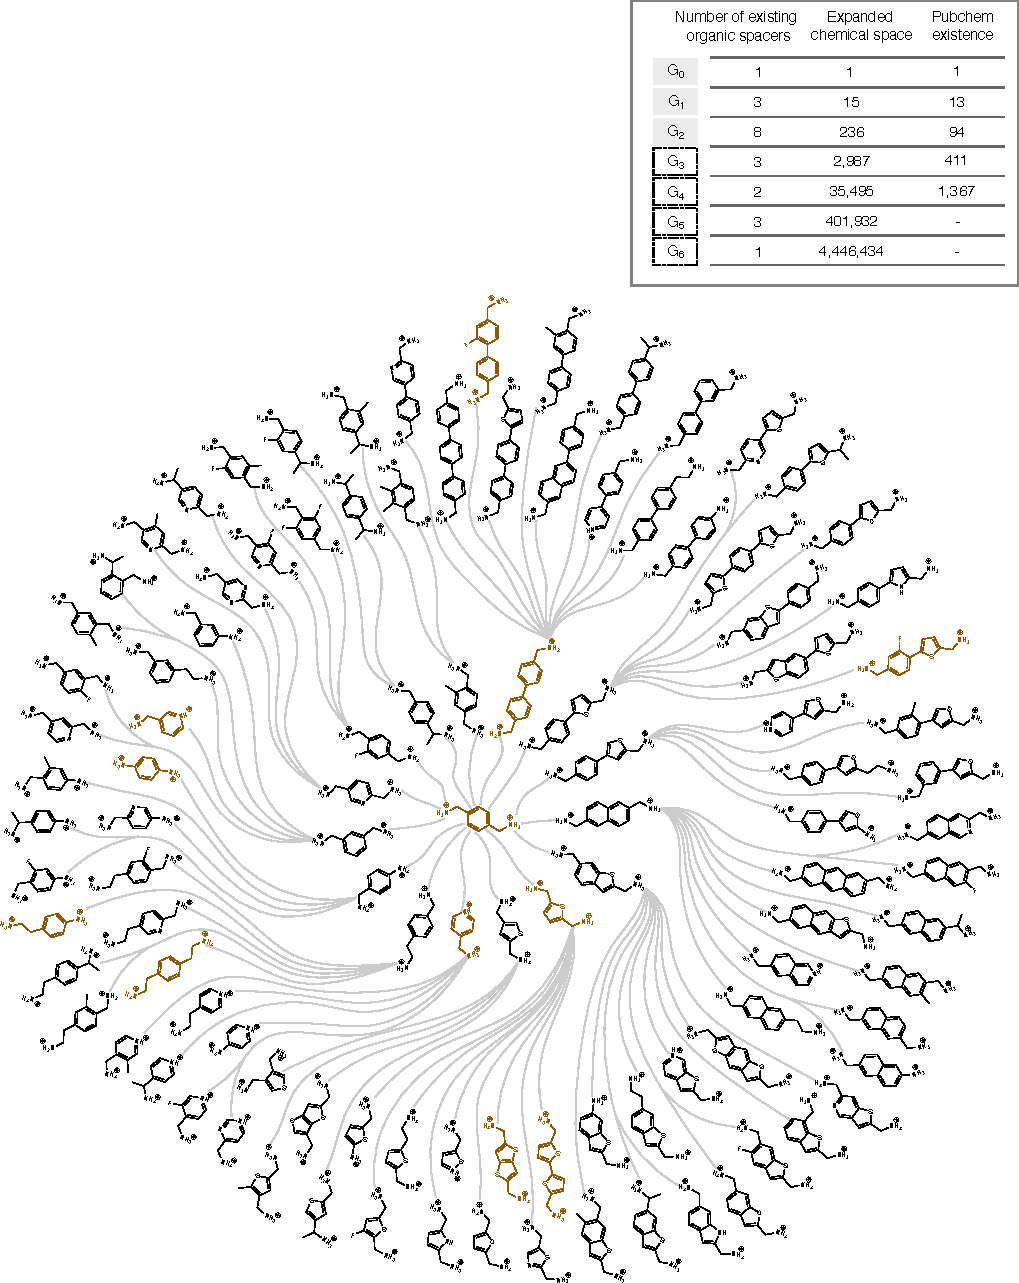
\includegraphics[width=\textwidth]{figures/HT-ML/figure4-1.pdf}
    \caption{Scaffold tree plot illustrating the organic spacer generation process.}
    \label{fig:figure4.1}
\end{figure}

To systematically explore a broad and diverse chemical space, we employed a deterministic molecular morphing approach rather than stochastic molecular generation methods\cite{RN236,RN310}. This ensures controlled diversification while maintaining the chemical interpretability of the generated spacers. As detailed in Chapter \ref{c:method}, each spacer is represented by a 12-digit fingerprint vector, which encodes key molecular features such as $\pi$-conjugation, ammonium tethering, heteroatom substitution, and side-chain modifications. All the morphing operators are associated with organic desciptors in the molecular fingerprint (Table \ref{t:morphing1}). This approach enables the enumeration of structurally diverse yet chemically meaningful molecular variations, ensuring a comprehensive and uniform coverage of the chemical space.

We initiate the morphing process from PDMA (Generation 0, $G_0$), a well-characterized organic spacer\cite{RN34}. We iteratively apply 13 distinct morphing operators to introduce incremental modifications, systematically generating higher-order generations ($G_1-G_6$). The molecular generation process is illustrated in Figure \ref{fig:figure4.1}. All organic spacers in $G_0$ (centre core), $G_1$(first circle) are displayed. For $G_2$ (second and third circle), only representative structures with unique molecular fingerprints to maintain clarity. Experimentally reported molecules within $G_0-G_2$ are highlighted, while the inset table quantifies the exponential expansion of the chemical space, which increases from an initial set of 21 reported organic spacers to millions of hypothetical spacers within $G_0-G_6$.

\begin{table}[!ht]
    \centering
    \caption{List of organic descriptors and their associated morphing operators.}\label{t:morphing1}
    \begin{tabular}{|l|r|r|}
        \hline
        \textbf{Number} & \textbf{Morphing operation} & \textbf{Organic descriptor} \\  \hline
        1 & Benzene-thiophene ring exchange & five-membered ring \\ \hline
        2 & Ring linkage & ring linkage \\ \hline 
        3 & Ring fusion & ring fusion \\ \hline
        4 & Primary secondary amine exchange & number of primary amine \\ \hline 
        5 & Linker length increase & Linker length \\ \hline 
        6 & Linker length decrease & Linker length \\ \hline
        7 & Linker position change & linker position \\  \hline
        8 & Hetero-nitrogen substitution & hetero-nitrogen \\  \hline 
        9 & Fluorination & fluorination \\  \hline
        10 & Furan exchange & furan \\ \hline 
        11 & Pyrrole exchange & pyrrole \\ \hline 
        12 & Side chain on backbone & no. side chain on backbone \\ \hline  
        13 & Side chain on linker & no. side chain on linker \\ \hline
    \end{tabular}
\end{table}

The morphing operations yield progressively complex sets of organic spacers. For example, to incorporate five-membered ring backbones, we utilize a ring contraction operator that transforms benzene into thiophene, thereby diversifying the core molecular framework. This systematic expansion extends beyond commonly studied phenyl- and thiophene-containing families, encompassing a broader spectrum of heteroatom-substituted structures (e.g., F, O, N) and various side-chain modifications.

The 21 experimentally reported organic spacers were captured within generations $G_0-G_6$, and with comparable complexity in these generations, we enumerated 21,306 fingerprints, corresponding to 4,887,100 hypothetical organic spacers. To assess the chemical feasibility of the generated molecules, the neutral forms of the hypothetical spacers were cross-referenced against the PubChem database. Within generations $G_0-G_4$, where computational feasibility allowed exhaustive searches, $\sim10^3$ spacers were identified in PubChem, confirming that a subset of our generated structures aligns with known chemical compounds. This validates the chemical plausibility of the generated molecular space.

\subsection{Visualization of generated chemical space}

To provide an intuitive understanding of the distribution and structural diversity of the generated organic spacers, we employ a dimensionality reduction technique to visualize the chemical space. Since the molecular fingerprints exist in a 12-dimensional space, we utilize t-distributed stochastic neighbour embedding (t-SNE)\cite{RN551}, an unsupervised learning algorithm that transforms high-dimensional data into a two-dimensional representation while preserving the relative distances between structurally similar molecules.

\begin{figure}[htbp]
    \centering
    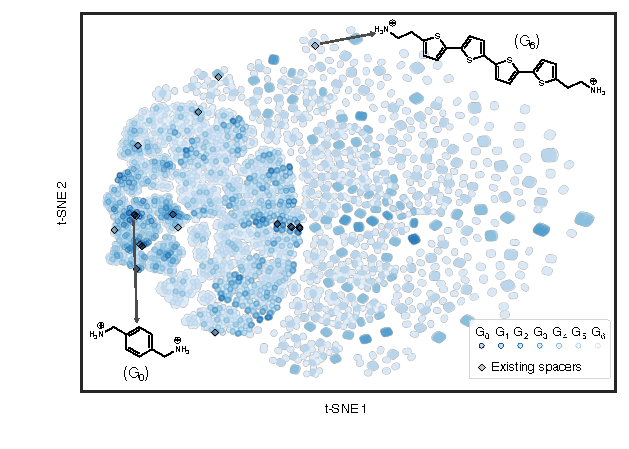
\includegraphics[width=0.8\textwidth]{figures/HT-ML/figure4-2.pdf}
    \caption{t-SNE representation of the generated chemical space containing the hypothetical organic spacers.}
    \label{fig:figure4.2}
\end{figure}

The resulting t-SNE map is shown in Figure \ref{fig:figure4.2}, representing $\sim2\times10^4$ unique fingerprints corresponding to $\sim4\times10^6$ organic spacers across generations $G_0-G_6$. Experimentally reported spacers are highlighted, with representative molecules from $G_0$ and $G_6$ explicitly labelled. The spatial organization of the t-SNE clusters reflects the underlying structural similarities among different spacers: closely grouped molecules share similar fingerprint features, while larger inter-cluster distances correspond to structurally dissimilar spacers.

Notably, among all reported spacers, the highest-generation example ($G_6$), AE4T\cite{RN38}, is distinctly separated from other spacers, reflecting its more complex structure. This visualization demonstrates that our generative workflow comprehensively covers the chemical space surrounding experimentally known spacers, including AE4T. Compared to traditional molecular datasets compiled from pre-existing databases, our approach ensures a more uniform and representative sampling, avoiding biases toward extreme or rare structures. By maintaining a balanced distribution of generated molecules, we enable reliable high-throughput calculations and robust machine learning predictions. As we will demonstrate later in this chapter, this curated dataset serves as a reliable foundation for training machine learning models, enhancing their ability to predict electronic properties with high accuracy.

\subsection{Descriptor-based visualization and cluster analysis}

\begin{figure}[htbp]
    \centering
    \includegraphics[width=\textwidth]{figures/HT-ML/figure4-3-1.pdf}
    \caption{Visualization of the chemical space with respect to organic descriptors in molecular fingerprint (Part 1).}
    \label{fig:figure4.3}
\end{figure}

\begin{figure}[htbp]
    \centering
    \ContinuedFloat
    \includegraphics[width=\textwidth]{figures/HT-ML/figure4-3-2.pdf}
    \caption{Visualization of the chemical space with respect to organic descriptors in molecular fingerprint (Part 2, continued).}
\end{figure}

To further examine the relationships between molecular descriptors and structural similarity, we present Figure \ref{fig:figure4.3}, which depicts the same t-SNE map but color-coded according to different molecular descriptors derived from the fingerprint vector. 
This visualization highlights key trends:
\begin{enumerate}
    \item Molecular spacers with similar descriptors cluster together, confirming that the fingerprint representation effectively captures structural relationships.
    \item The non-linear characteristic of t-SNE is well observed and it makes it easier to understand how t-SNE work. Note that the non-linearity organization of data points reflects the fundamental difference between t-SNE and principal component analysis (PCA). While PCA, a linear dimensionality reduction technique, is widely used in materials informatics, we found that it resulted in excessive overlap between structurally distinct molecules. By contrast, t-SNE preserves local structures more effectively, providing better differentiation of organic spacers.
\end{enumerate}

\begin{figure}[htbp]
    \centering
    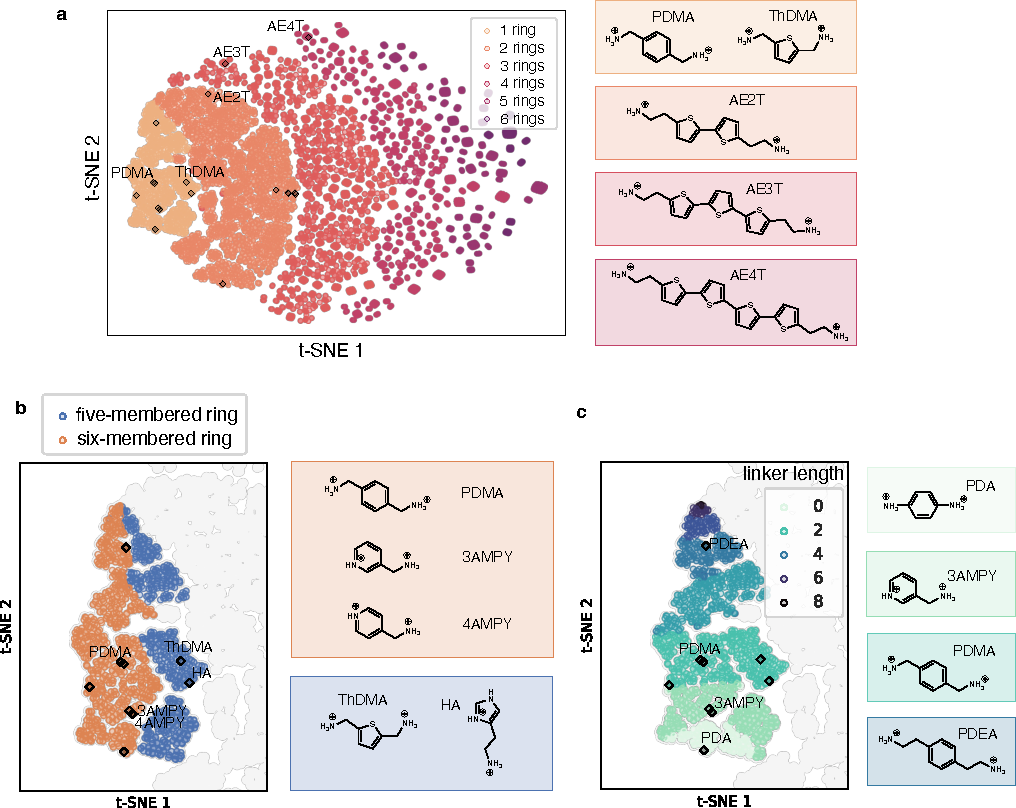
\includegraphics[width=\textwidth]{figures/HT-ML/figure4-4.pdf}
    \caption[Chemical space visualization of existing spacers.]{Chemical space visualization of existing spacers. \textbf{a} Complete chemical space. \textbf{b,c} Enlarged views highlighting spacers containing a single aromatic ring.}
    \label{fig:figure4.4}
\end{figure}


A deeper analysis of specific clusters within the t-SNE map is presented in Figure \ref{fig:figure4.4}, focusing on the existing organic spacers. The full distribution of the generated organic spacers is shown in Figure \ref{fig:figure4.4}a. A clear gradient is observed from left to right, reflecting increasing number of aromatic rings. Spacers such as PDMA and ThDMA, which contain a single aromatic ring and are widely used in 2D perovskites, cluster on the left side of the plot. On the other hand, highly conjugated organic spacers, such as the oligothiophene-based spacers (AE2T, AE3T, AE4T) are found progressively further to the right.

Figure \ref{fig:figure4.4} b,c provide focused views of subspaces containing spacers with a single aromatic ring. In \textbf{b}, molecules are colored by ring type, highlighting distinct clustering between five-membered ring and six-membered ring as conjugated backbones. In \textbf{c}, the same subset is colored by linker length. A spatial gradient is visible, with shorter linkers (e.g., PDA, linker length = 0) clustering in the top and longer linkers (e.g., PDEA, linker length = 4) spreading toward the bottom. This demonstrates that the fingerprint-based t-SNE projection effectively captures meaningful structural and functional diversity among known spacers.



\section{Influence of organic spacer structure on energy levels}\label{section:section4-2}

\subsection{DFT calculation of DJ perovskites}

To assess the impact of organic spacer selection on the electronic properties of DJ perovskites, we performed a detailed high-throughput DFT analysis on 261 DJ-phase perovskites. This dataset includes both experimentally reported spacers and hypothetical spacers from generations $G_0-G_2$ of our expanded chemical space. Model crystal structures were constructed by inserting organic spacers between the PbI$_4$ layers, with each unit cell containing four diammonium spacers and four PbI$_4$ units (see Chapter \ref{c:method} for computational details). 

\textbf{Organic spacer packing configurations}

In computational studies of DJ perovskites, two primary packing arrangements of organic spacers are typically assumed: in-phase and out-of-phase configurations. Unlike the inorganic sublattice, which undergoes significant structural distortions (such as octahedral tilting and bond-angle variations), the organic spacers exhibit minimal changes in packing pattern upon structural relaxation. This behaviour suggests that interactions between organic spacers and the inorganic layers, as well as interactions among the organic spacers themselves, are relatively weak, occurring primarily through hydrogen bonding and van der Waals interactions. Consequently, both in-phase and out-of-phase arrangements lead to well-converged structures, indicating that the energy difference between these configurations is small. This suggests a shallow energy landscape with respect to the relative alignment of organic spacers.

Despite the energetic similarity between different packing arrangements, our analysis revealed that the packing configuration has minimal influence on the energy level alignment. Therefore, to align with experimentally observed structures, all organic spacers were assign to arranged in herringbone (out-of-phase) configurations\cite{RN41}. The optimized geometries were computed at the DFT-PBE level. 

\textbf{Bandgap calibration and energy level alignment}

The energy level alignment between the organic frontier molecular orbitals and the inorganic band edges was subsequently determined using HSE + SOC calculations. A key parameter influencing the computed bandgap values is the mixing factor, which defines the fraction of exact exchange in the hybrid functional. Previous studies on 2D perovskites have used mixing factors ranging from 0.25 to 0.45 to match experimental bandgaps. Our calculations confirm that while the choice of mixing factor significantly alters absolute bandgap values, its impact on energy level alignment trends is minimal, as both organic and inorganic components exhibit a similar response to changes in the mixing factor.
To ensure consistency with experimental data, we benchmarked our DFT results against available experimental bandgap values, finding that a mixing factor of 0.4 provided the best agreement (see Chapter \ref{c:method} for further discussion).

\textbf{Energy level trends in DJ perovskites}

\begin{figure}[htbp]
    \centering
    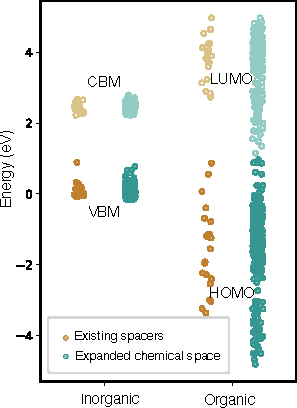
\includegraphics[width=0.5\textwidth]{figures/HT-ML/figure4-5.pdf}
    \caption{Energy level alignment in DJ perovskites with existing spacers and hypothetical organic spacers.}
    \label{fig:figure4.5}
\end{figure}

Our analysis revealed that the majority of DJ perovskites (18 out of 21 experimentally reported structures) exhibit type Ia energy level alignment, characterized by low-energy electrons and holes localized in inorganic layers. The remaining three structures exhibit type IIa alignment. The primary factor dictating this variation in energy level alignment is the frontier molecular orbitals levels of the organic spacers, which exhibit a broad energy variation of $\sim6.1$ eV. In contrast, the inorganic band edges remain relatively invariant, with a variation of only $\sim0.9$ eV (see Figure \ref{fig:figure4.5}). This observation aligns with the common approximation cited in the literature that inorganic energy levels of 2D perovskites can be assumed unchanged with different organic spacers\cite{RN18,RN20}. 

Furthermore, Figure \ref{fig:figure4.5} illustrates how our expanded chemical space exploration has significantly extended the range of organic frontier levels compared to previous studies. The generated DJ perovskites—including $G_0-G_2$ and inverse designed final candidates (introduced later in Chapter \ref{c:result-2})—exhibit an expanded energy distribution of organic frontier levels, covering a much wider range than the reported organic spacers, underscoring the effectiveness of our chemical space exploration approach. 

\subsection{Four factors governing energy level alignment}

\begin{figure}[htbp]
    \centering
    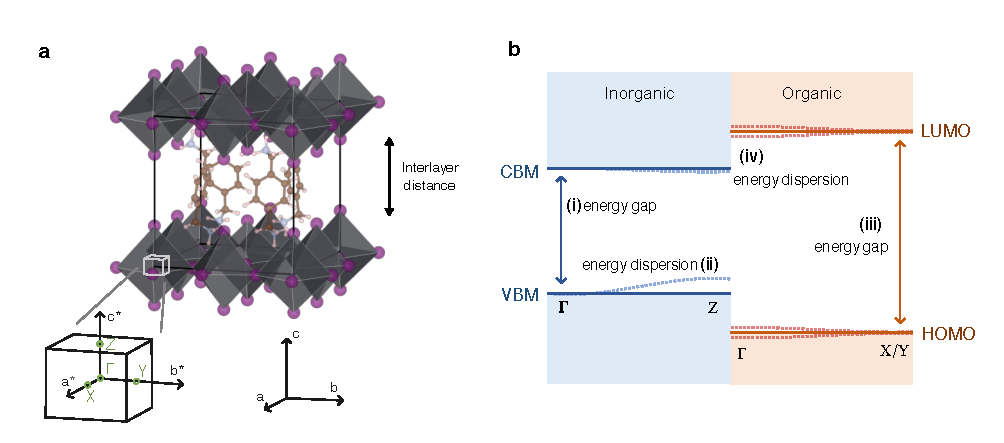
\includegraphics[width=\textwidth]{figures/HT-ML/figure4-6.pdf}
    \caption{Four factors affecting the energy level alignment in DJ perovskites.}
    \label{fig:figure4.6}
\end{figure}

To further understand the structure-property relationships governing energy level alignment in DJ perovskites, we analysed key electronic band structure trends across all structures studied. Four dominant factors were identified, as illustrated in Figure \ref{fig:figure4.6}:

(i) Energy gap at the inorganic band edge ($\Gamma$ point)

(ii) Inorganic band dispersion along the stacking direction ($\Gamma$ to $Z$)

(iii) Energy gap between the organic frontier orbitals (HOMO-LUMO levels)

(iii) Frontier orbital dispersion of the organic spacers

\textbf{Electronic structure of inorganic component}

\begin{figure}[htbp]
    \centering
    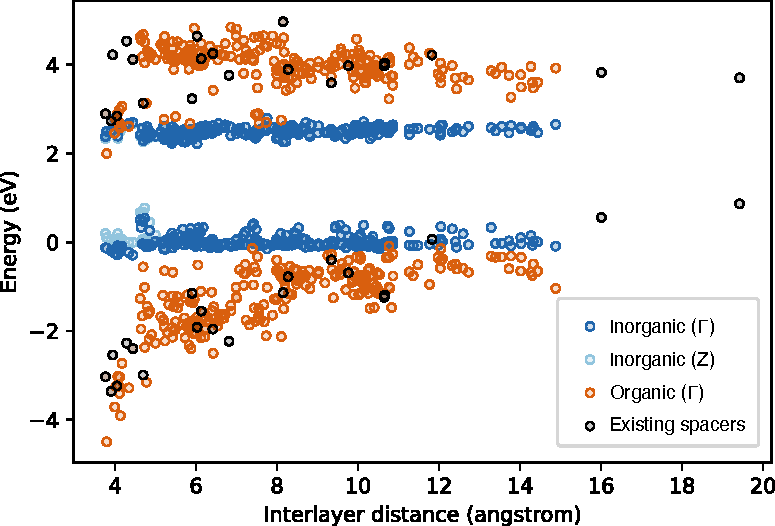
\includegraphics[width=0.9\textwidth]{figures/HT-ML/figure4-7.pdf}
    \caption{Energy level alignment in calculated DJ perovskites plotted against interlayer distance.}
    \label{fig:figure4.7}
\end{figure}

The inorganic layers in DJ perovskites typically form direct bandgap semiconductors with their valence band maximum (VBM) and conduction band minimum (CBM) located at the $\Gamma$ point in the Brillouin zone. However, in cases where interlayer coupling is significant, the bandgap shifts to the Z point. 

The band dispersion is strongly anisotropic, exhibiting strong dispersion in the $\Gamma-X/Y$ direction (in-plane directions in real space), while the dispersion in the $\Gamma-Z$ direction (stacking direction) depends on interlayer interactions. This trend of interlayer interaction is illustrated in Figure \ref{fig:figure4.7}, where the energy level alignment is plotted against the interlayer distance. Interlayer coupling, characterized by the energy difference between the $\Gamma$ and $Z$ point of the inorganic band edge, becomes significant only when the interlayer distance is relatively small.

\begin{figure}[htbp]
    \centering
    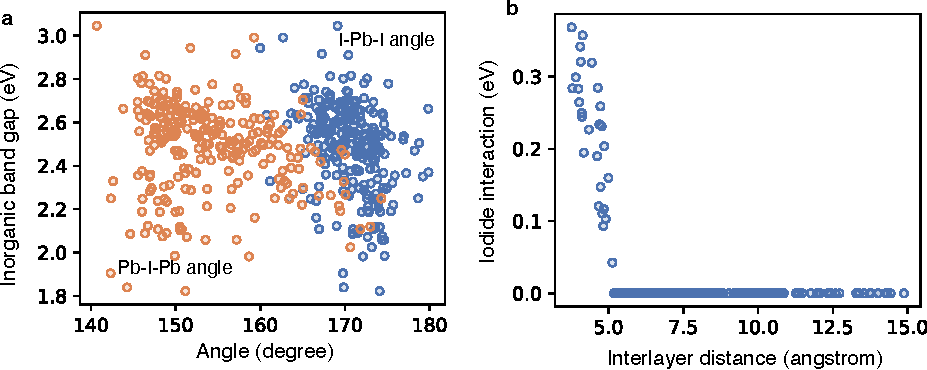
\includegraphics[width=\textwidth]{figures/HT-ML/figure4-8.pdf}
    \caption{Indirect influence of organic spacers on inorganic band edges.}
    \label{fig:figure4.8}
\end{figure}

To further quantify the structure-property relationship between inorganic framework geometry and energy levels, we examined two key structural factors (Figure \ref{fig:figure4.8}):

\begin{itemize}
    \item Factor (i) in Figure \ref{fig:figure4.6} is mainly affected by octahedral tilting and distortion. As shown in Figure \ref{fig:figure4.8}a, variations in the Pb-I-Pb bond angle and I-Pb-I internal distortion significantly impact the inorganic energy gap at the $\Gamma$ point, leading to energy shifts of approximately 1 eV. These distortions arise due to hydrogen bonding interactions between the PbI$_6$ octahedra and the organic cations.
    \item Factor (ii) in Figure \ref{fig:figure4.6} is mainly affected by interlayer distance. As shown in Figure \ref{fig:figure4.8}b, when the interlayer distance decreases below 5.0 $\AA$, iodide-iodide interactions enhance $\Gamma-Z$ energy dispersion, also inducing $\sim$1 eV energy shifts. This behaviour is commonly observed in DJ-phase perovskites with short organic spacers and is consistent with trends reported in ACI-phase perovskites\cite{RN242,RN31}.
\end{itemize}

\textbf{Electronic structure of the organic component}

Unlike the band-like behaviour of the inorganic layers, the organic frontier orbitals (HOMO and LUMO) remain localized and discrete, with minimal dispersion, closely resembling their isolated molecular forms. This occurs because:
\begin{itemize}
    \item There is not interlayer interaction between organic spacers in adjacent layers, resulting in zero dispersion along the $\Gamma-Z$ direction. 
    \item The in-plane ($\Gamma-X/Y$) dispersion is also minimal due to the herringbone packing of organic spacers, which restricts electronic interactions between adjacent organic units. More detailed discussions on the relationship between packing pattern and in-plane dispersion can be found in Chapter \ref{c:method}.
\end{itemize}

\subsection{Simplified modelling of organic frontier levels}

Our analysis confirms that the primary influence of organic spacers on DJ perovskite energy levels lies in their HOMO and LUMO levels, which is primarily a consequence of weak bonding interactions between organic cations and the inorganic framework\cite{RN42,RN144}. 

However, the high computational cost of DFT calculations for large DJ perovskite unit cells limits our ability to simulate thousands of structures. To address this, we propose an efficient approximation: Organic frontier energy levels in hybrid perovskites can be estimated using calculations on isolated cations.

\begin{figure}[htbp]
    \centering
    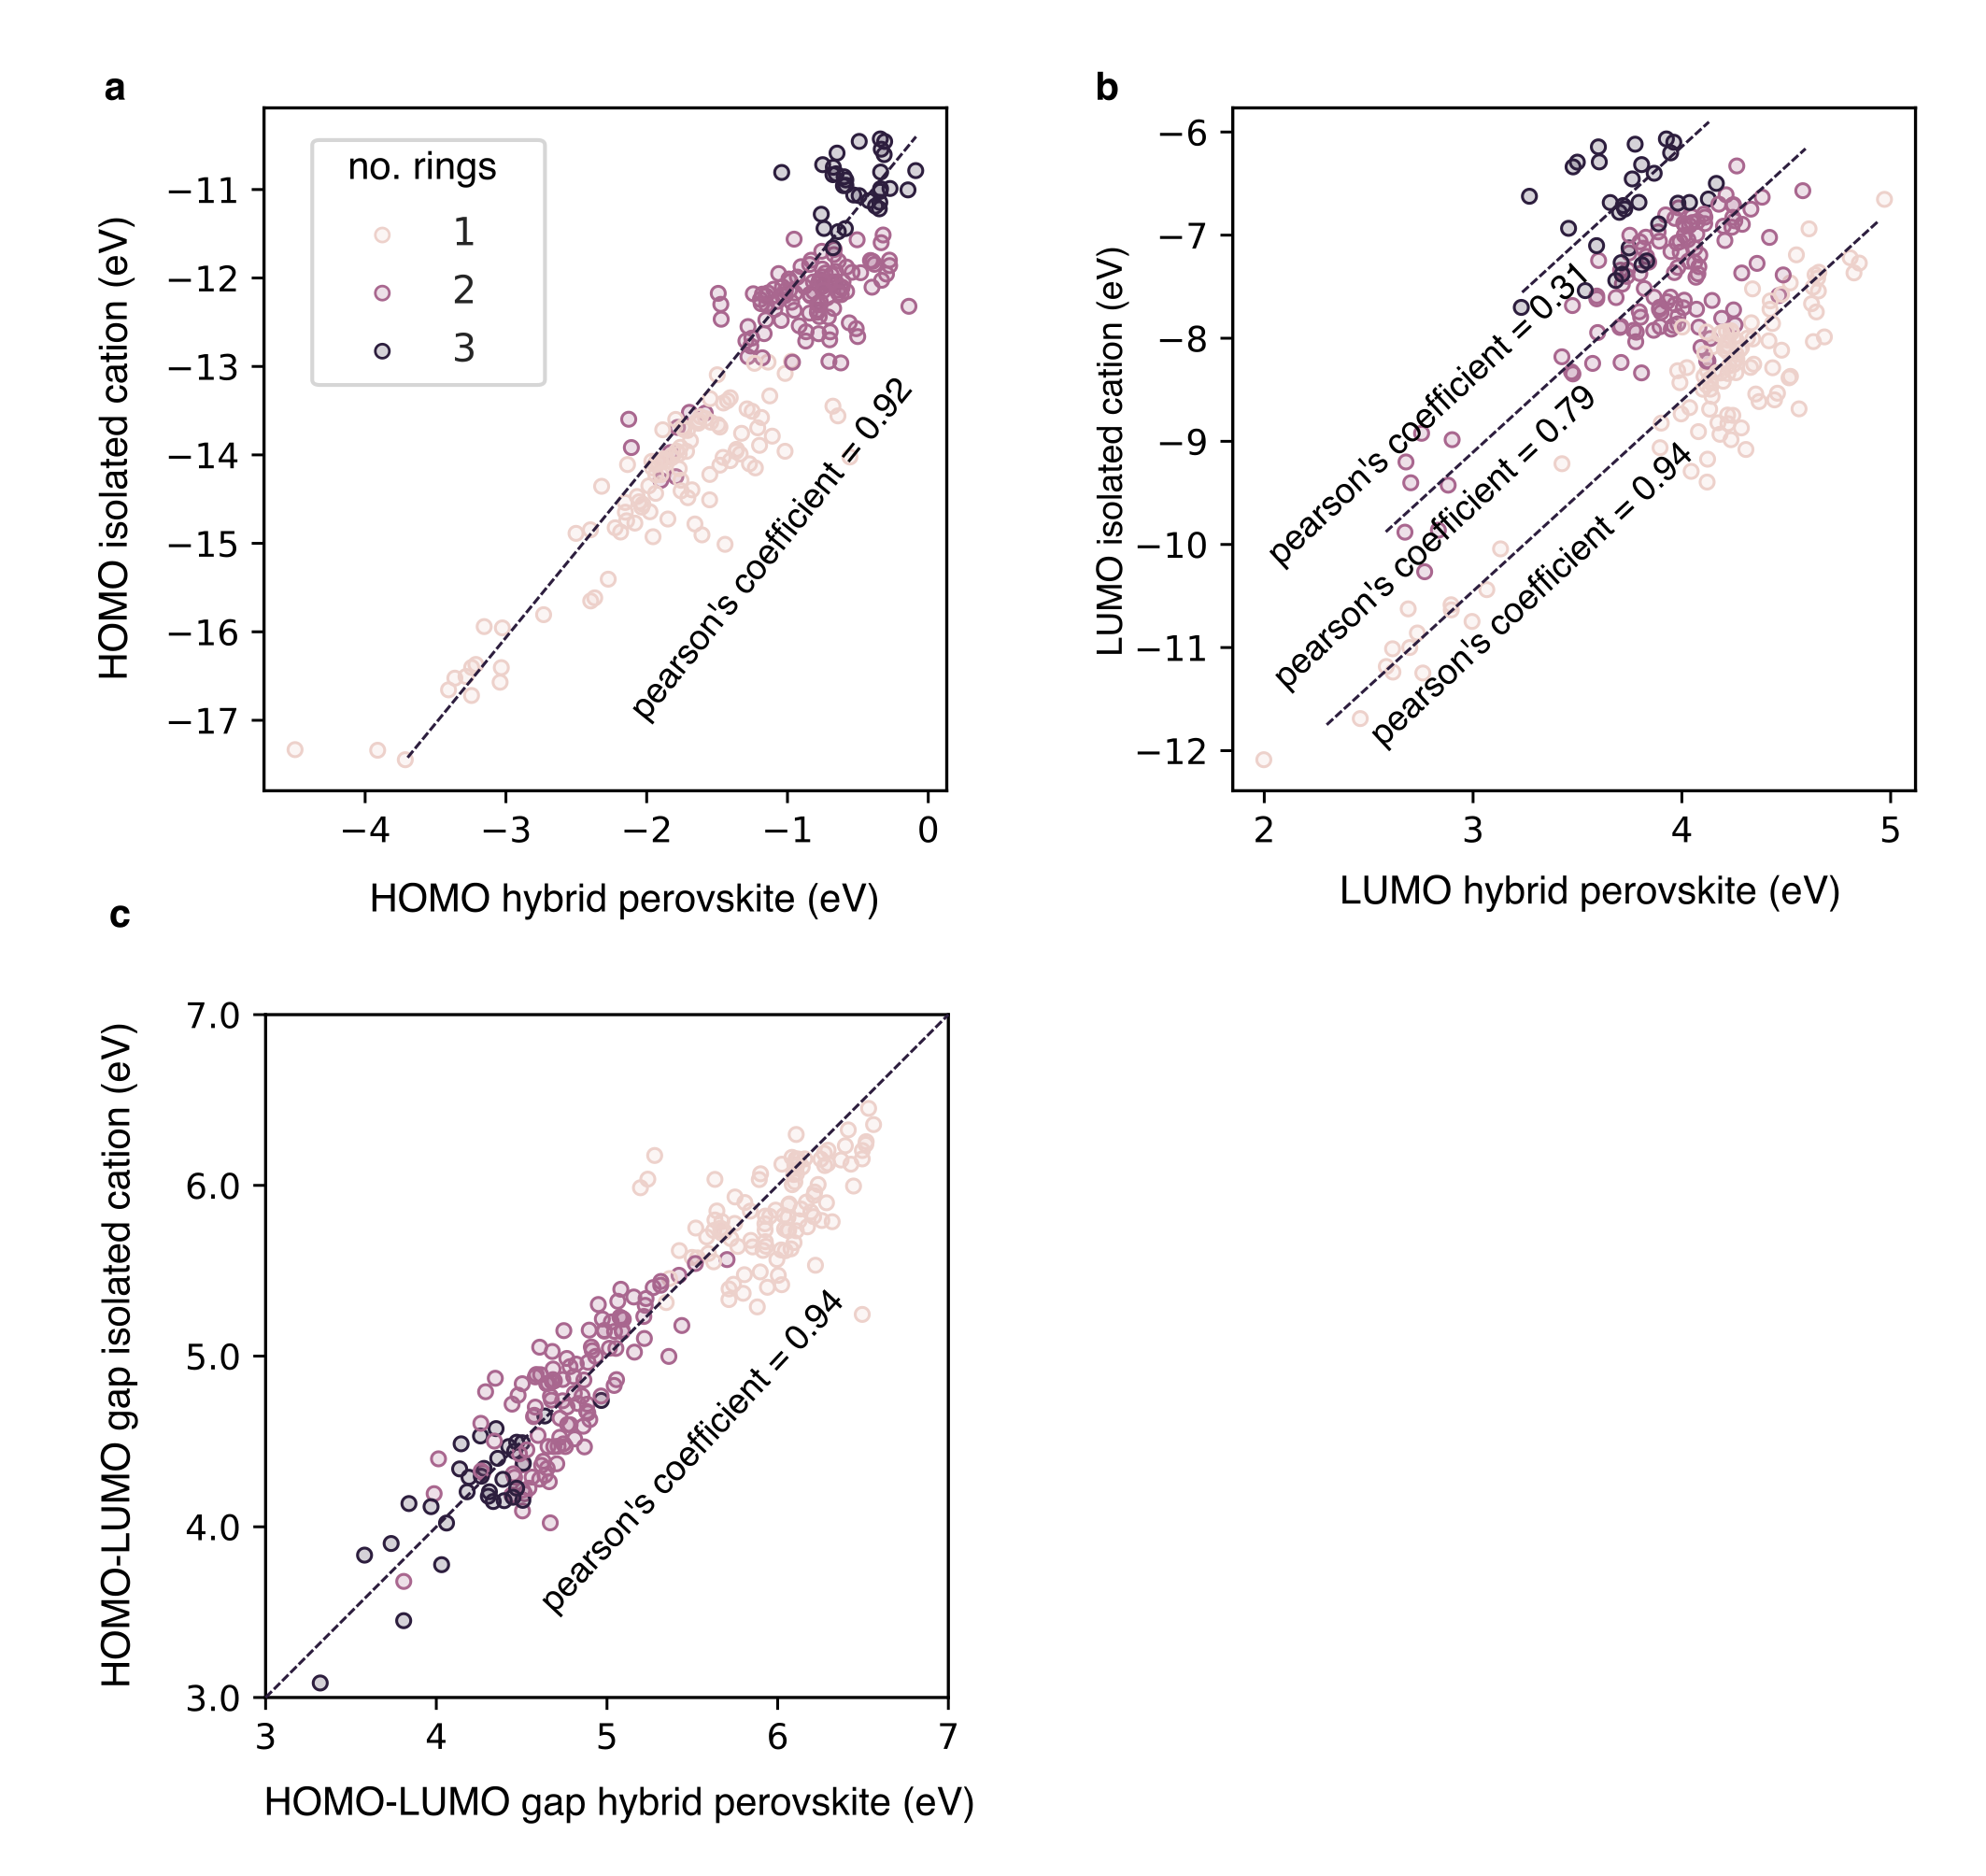
\includegraphics[width=\textwidth]{figures/HT-ML/figure4-9.png}
    \caption{Correlation between organic frontier levels in hybrid perovskites and their isolated molecular forms.}
    \label{fig:figure4.9}
\end{figure}

We computed frontier levels of isolated organic spacers using the B3LYP functional in Gaussian. Figure \ref{fig:figure4.9} compares the frontier orbital energies obtained from hybrid perovskite calculations and isolated organic cations. While absolute energy values differ because of functional choices, basis sets, and the chemical environment, a near-linear relationship emerges between the two calculations:

\begin{itemize}
    \item Figure \ref{fig:figure4.9}a shows that HOMO levels exhibit a linear correlation between hybrid perovskites and their isolated cation counterparts.
    \item Figure \ref{fig:figure4.9}b highlights a similar trend in LUMO levels, with noticeable dependence on the ring count of the organic spacer.
    \item Figure \ref{fig:figure4.9}c indicates that indicates that the HOMO–LUMO gap remains consistent between the two methods.
    
\end{itemize}

By leveraging these correlations, we can predict organic frontier levels without the need for fully relaxed DJ perovskite calculations for each candidate spacer. This significantly reduces the computational cost, enabling us to scale from hundreds to thousands of hypothetical structures—an essential step for generating robust datasets to train machine learning models in the subsequent sections.

\section{Selection and evaluation of machine learning models}\label{section:section4-3}

In the previous sections, we established how organic spacers affect the energy level alignment in DJ perovskites, and we identified key structural descriptors that can serve as input features for predictive modelling. Here, we describe how ML is employed to capture the structure–property relationships between molecular fingerprints and their frontier energy levels, and facilitate the rapid identification of promising spacer candidates.

\subsection{Molecular fingerprint as input feature}

\begin{figure}[htbp]
    \centering
    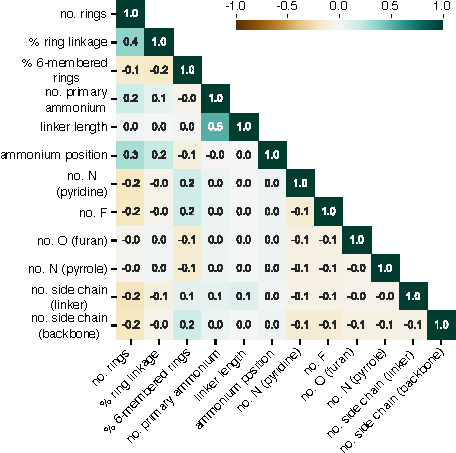
\includegraphics[width=0.9\textwidth]{figures/HT-ML/figure4-10.pdf}
    \caption{Correlation matrix of organic descriptors in the molecular fingerprint.}
    \label{fig:figure4.10}
\end{figure}

To represent each organic spacer, we use a 12-digit molecular fingerprint as the input feature for our machine learning pipeline. This fingerprint does not require additional feature selection, as it was specifically designed to minimize redundancy among descriptors. Indeed, Pearson’s correlation coefficients between fingerprint descriptors are all below 0.5 (see Figure \ref{fig:figure4.10}), confirming low inter-feature correlation and justifying the direct inclusion of all 12 features in model training. This is a significant advantage compared to previous studies that rely on diverse chemical descriptors and require feature selection to reduce multicollinearity\cite{RN315,RN283}.

Our machine learning dataset consists of 3,239 organic spacers spanning generations $G_0-G_3$, with HOMO/LUMO values from high-throughput calculations serving as the target properties. This dataset allows us to explore a broad range of structures and electronic characteristics, setting the stage for robust model training.

\subsection{Comparison of different models}

\begin{figure}[htbp]
    \centering
    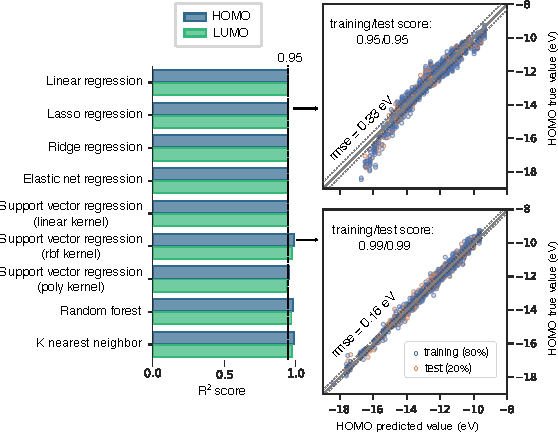
\includegraphics[width=\textwidth]{figures/HT-ML/figure4-11.pdf}
    \caption{Summary of ML model performance for HOMO/LUMO prediction.}
    \label{fig:figure4.11}
\end{figure}

\begin{figure}[htbp]
    \centering
    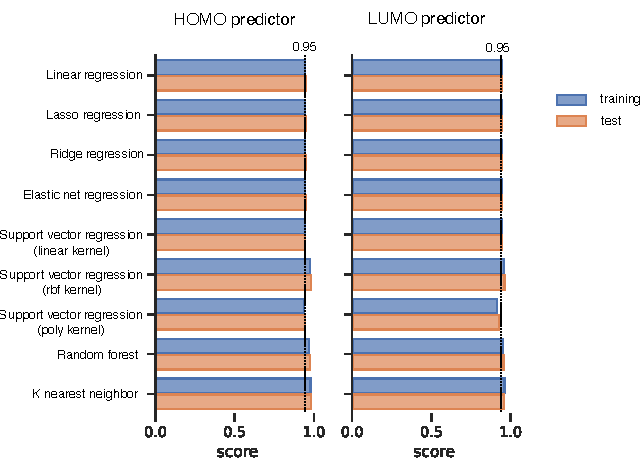
\includegraphics[width=0.9\textwidth]{figures/HT-ML/figure4-12.pdf}
    \caption{Comparison of training/test scores of various ML models for HOMO/LUMO prediction.}
    \label{fig:figure4.12}
\end{figure}

Because our goal is to predict HOMO and LUMO energies from known labels (i.e., computed frontier levels), this is a supervised regression problem. We trained separate machine learning models for HOMO and LUMO predictions respectively, with the dataset split into training and testing sets (80: 20 ratios). All models were evaluated using 15-fold cross-validation to ensure consistent and reliable estimation of fitting error. A variety of linear and non-linear regression methods commonly used in materials science literature were benchmarked, including:
\begin{itemize}
    \item Linear models: linear regression, LASSO regression, Ridge regression, Elastic net regression, Support vector regression with a linear kernel.

    \item Non-linear models: Random Forest, K nearest neighbour, Support Vector Regression with radial basis function (rbf) kernel or polynomial kernel. 
\end{itemize}

Figure \ref{fig:figure4.11} summarizes the R$^2$ scores (ranging from 0 to 1, with higher values indicating better predictions) for each model. Across both HOMO and LUMO predictions, nonlinear models achieve slightly higher R$^2$ scores (around 0.99/0.97) than linear models (around 0.95/0.95). Notably, no overfitting was detected, as evidenced by comparable performance on both training and test sets (Figure \ref{fig:figure4.12}).

Despite their slightly lower performance for low-energy frontier levels, linear models capture the overall trend effectively. This difference becomes clearer in Figure \ref{fig:figure4.13} (HOMO) and Figure \ref{fig:figure4.14} (LUMO), which plot predicted vs. true energy values alongside model scores and root mean squared errors (RMSE). While nonlinear models better capture the extreme regions of energy, linear models show no significant deviations from the overall relationship.

Since our primary objective was to classify energy level alignment types (e.g., Type Ia, Type IIa, etc.) rather than predict absolute HOMO/LUMO values, a slight accuracy gap at the extremes is not critical. By optimizing the decision boundary, linear models can serve as a highly interpretable alternative without a significant loss in performance. Consequently, linear models are chosen for subsequent analysis and feature interpretation.

\begin{figure}[htbp]
    \centering
    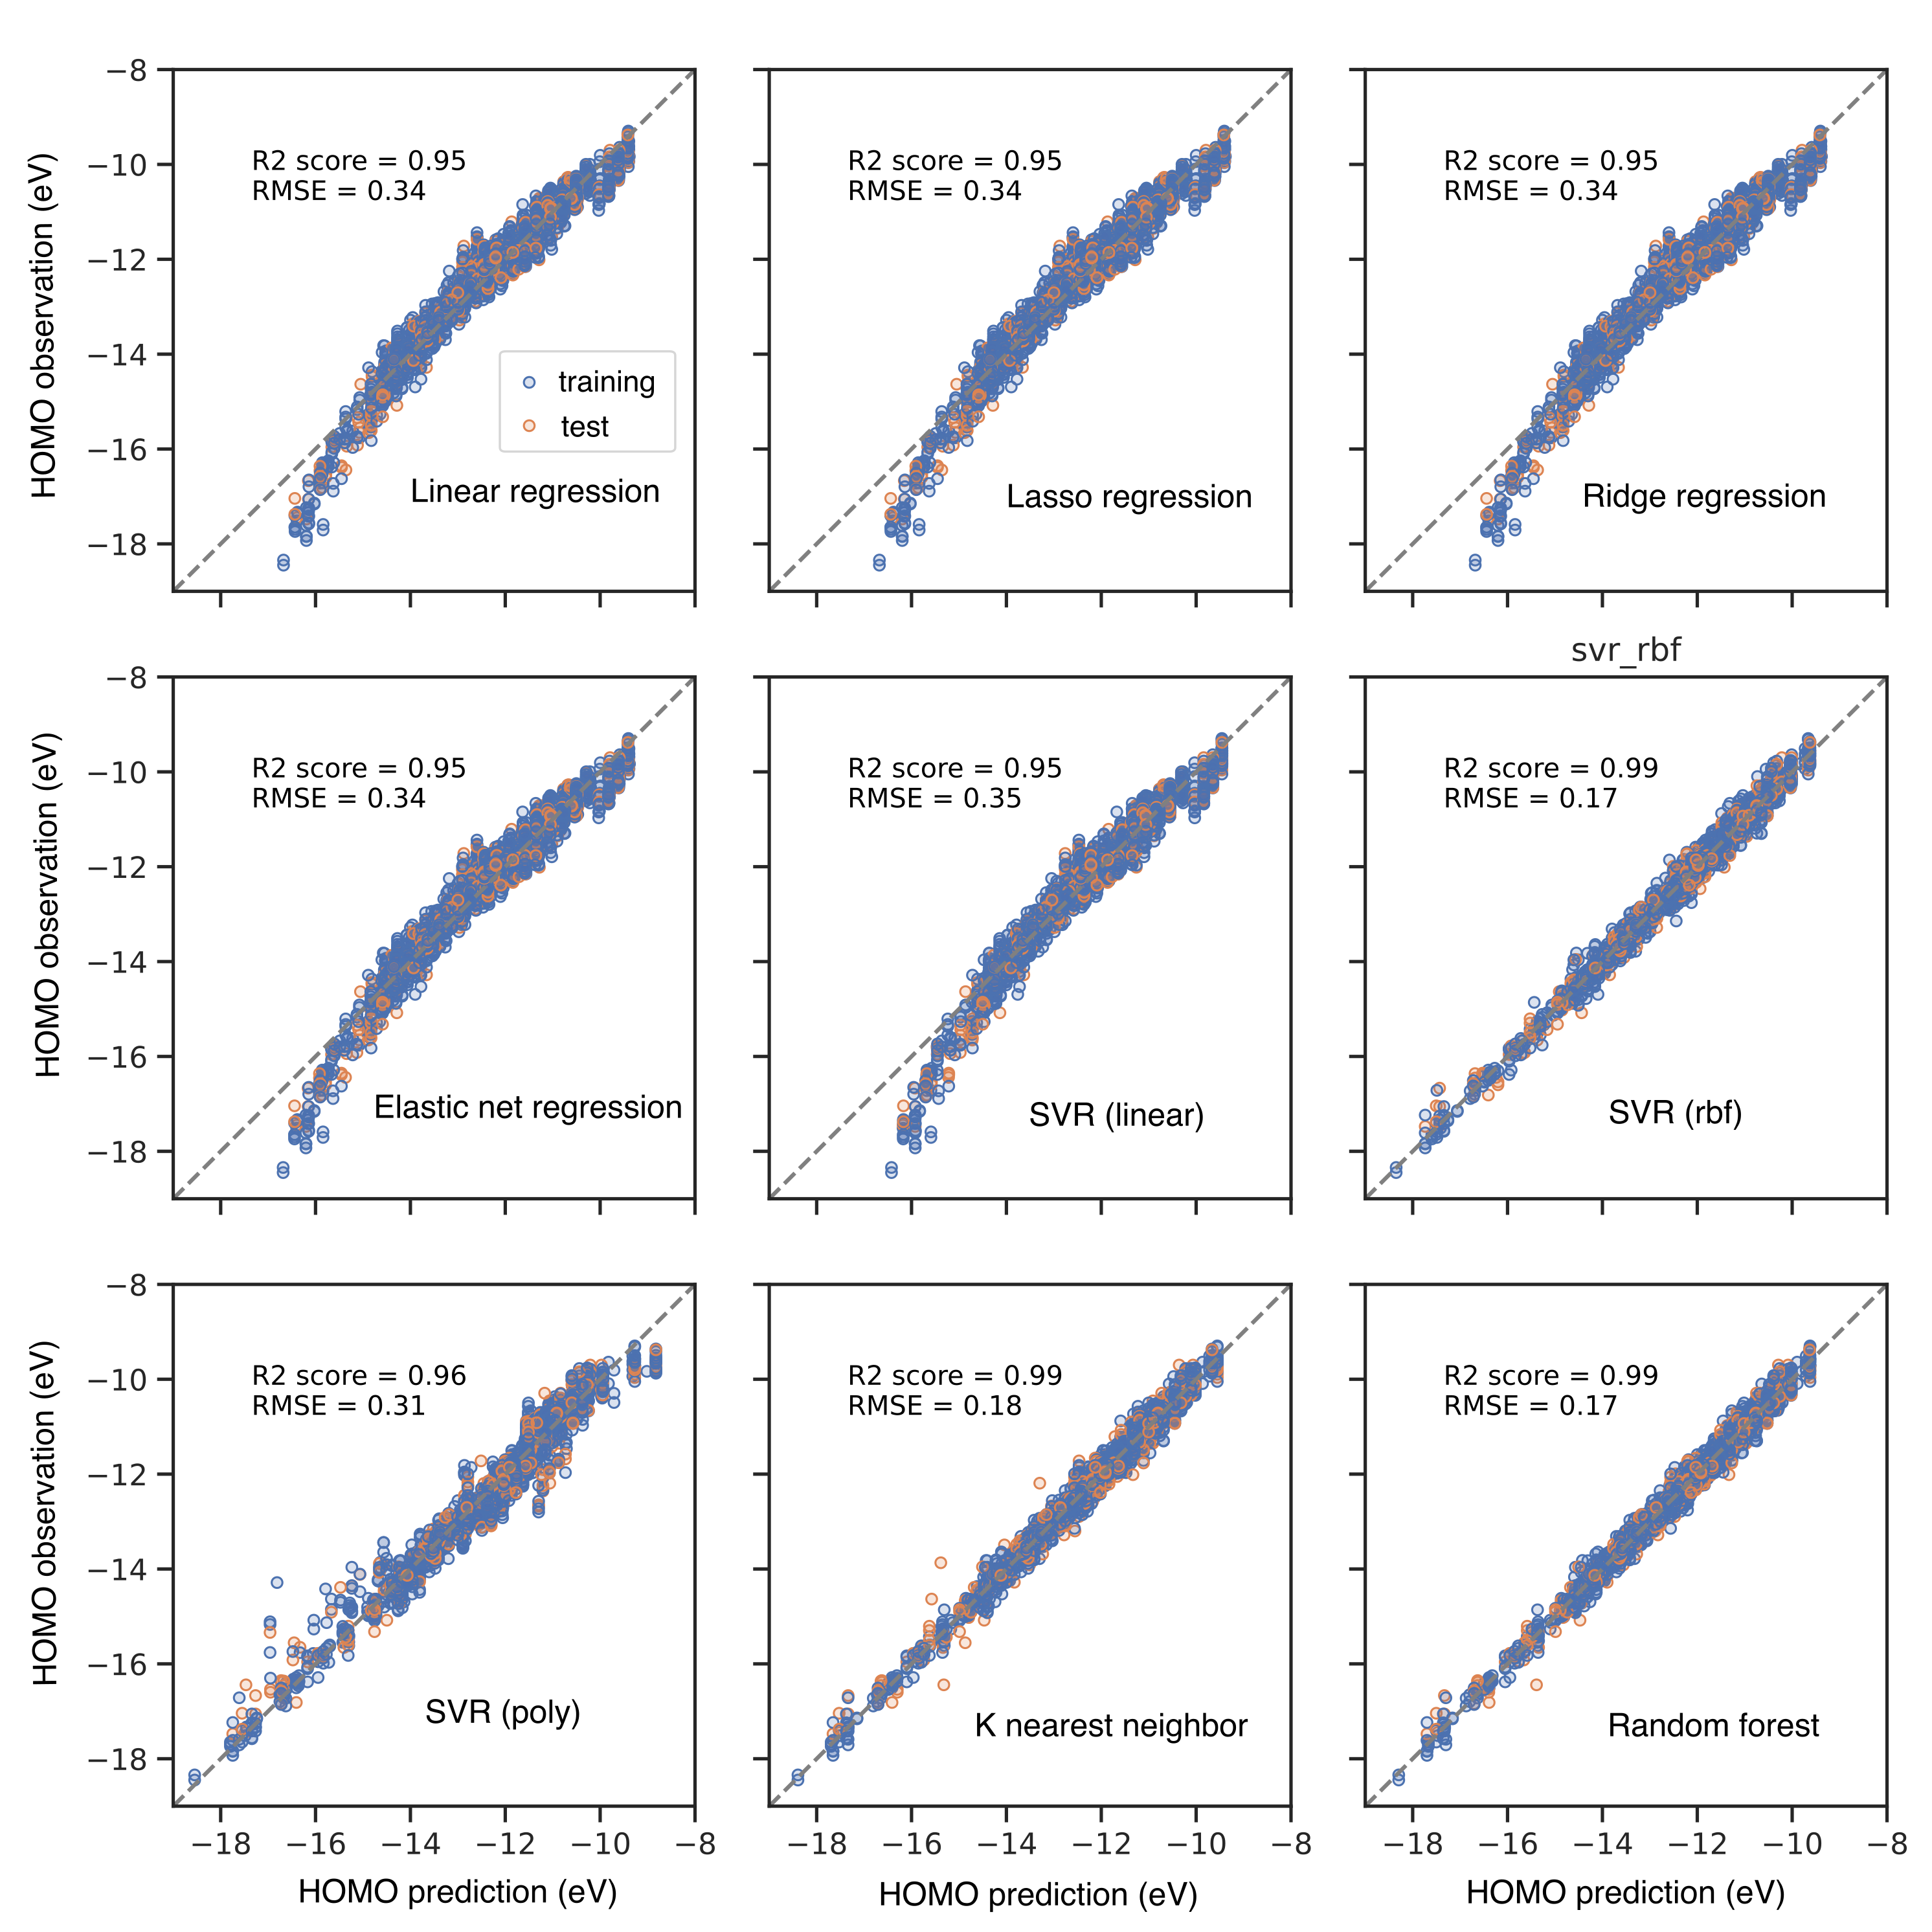
\includegraphics[width=\textwidth]{figures/HT-ML/figure4-13.png}
    \caption{Predicted vs. true values for HOMO level across various ML models.}
    \label{fig:figure4.13}
\end{figure}

\begin{figure}[htbp]
    \centering
    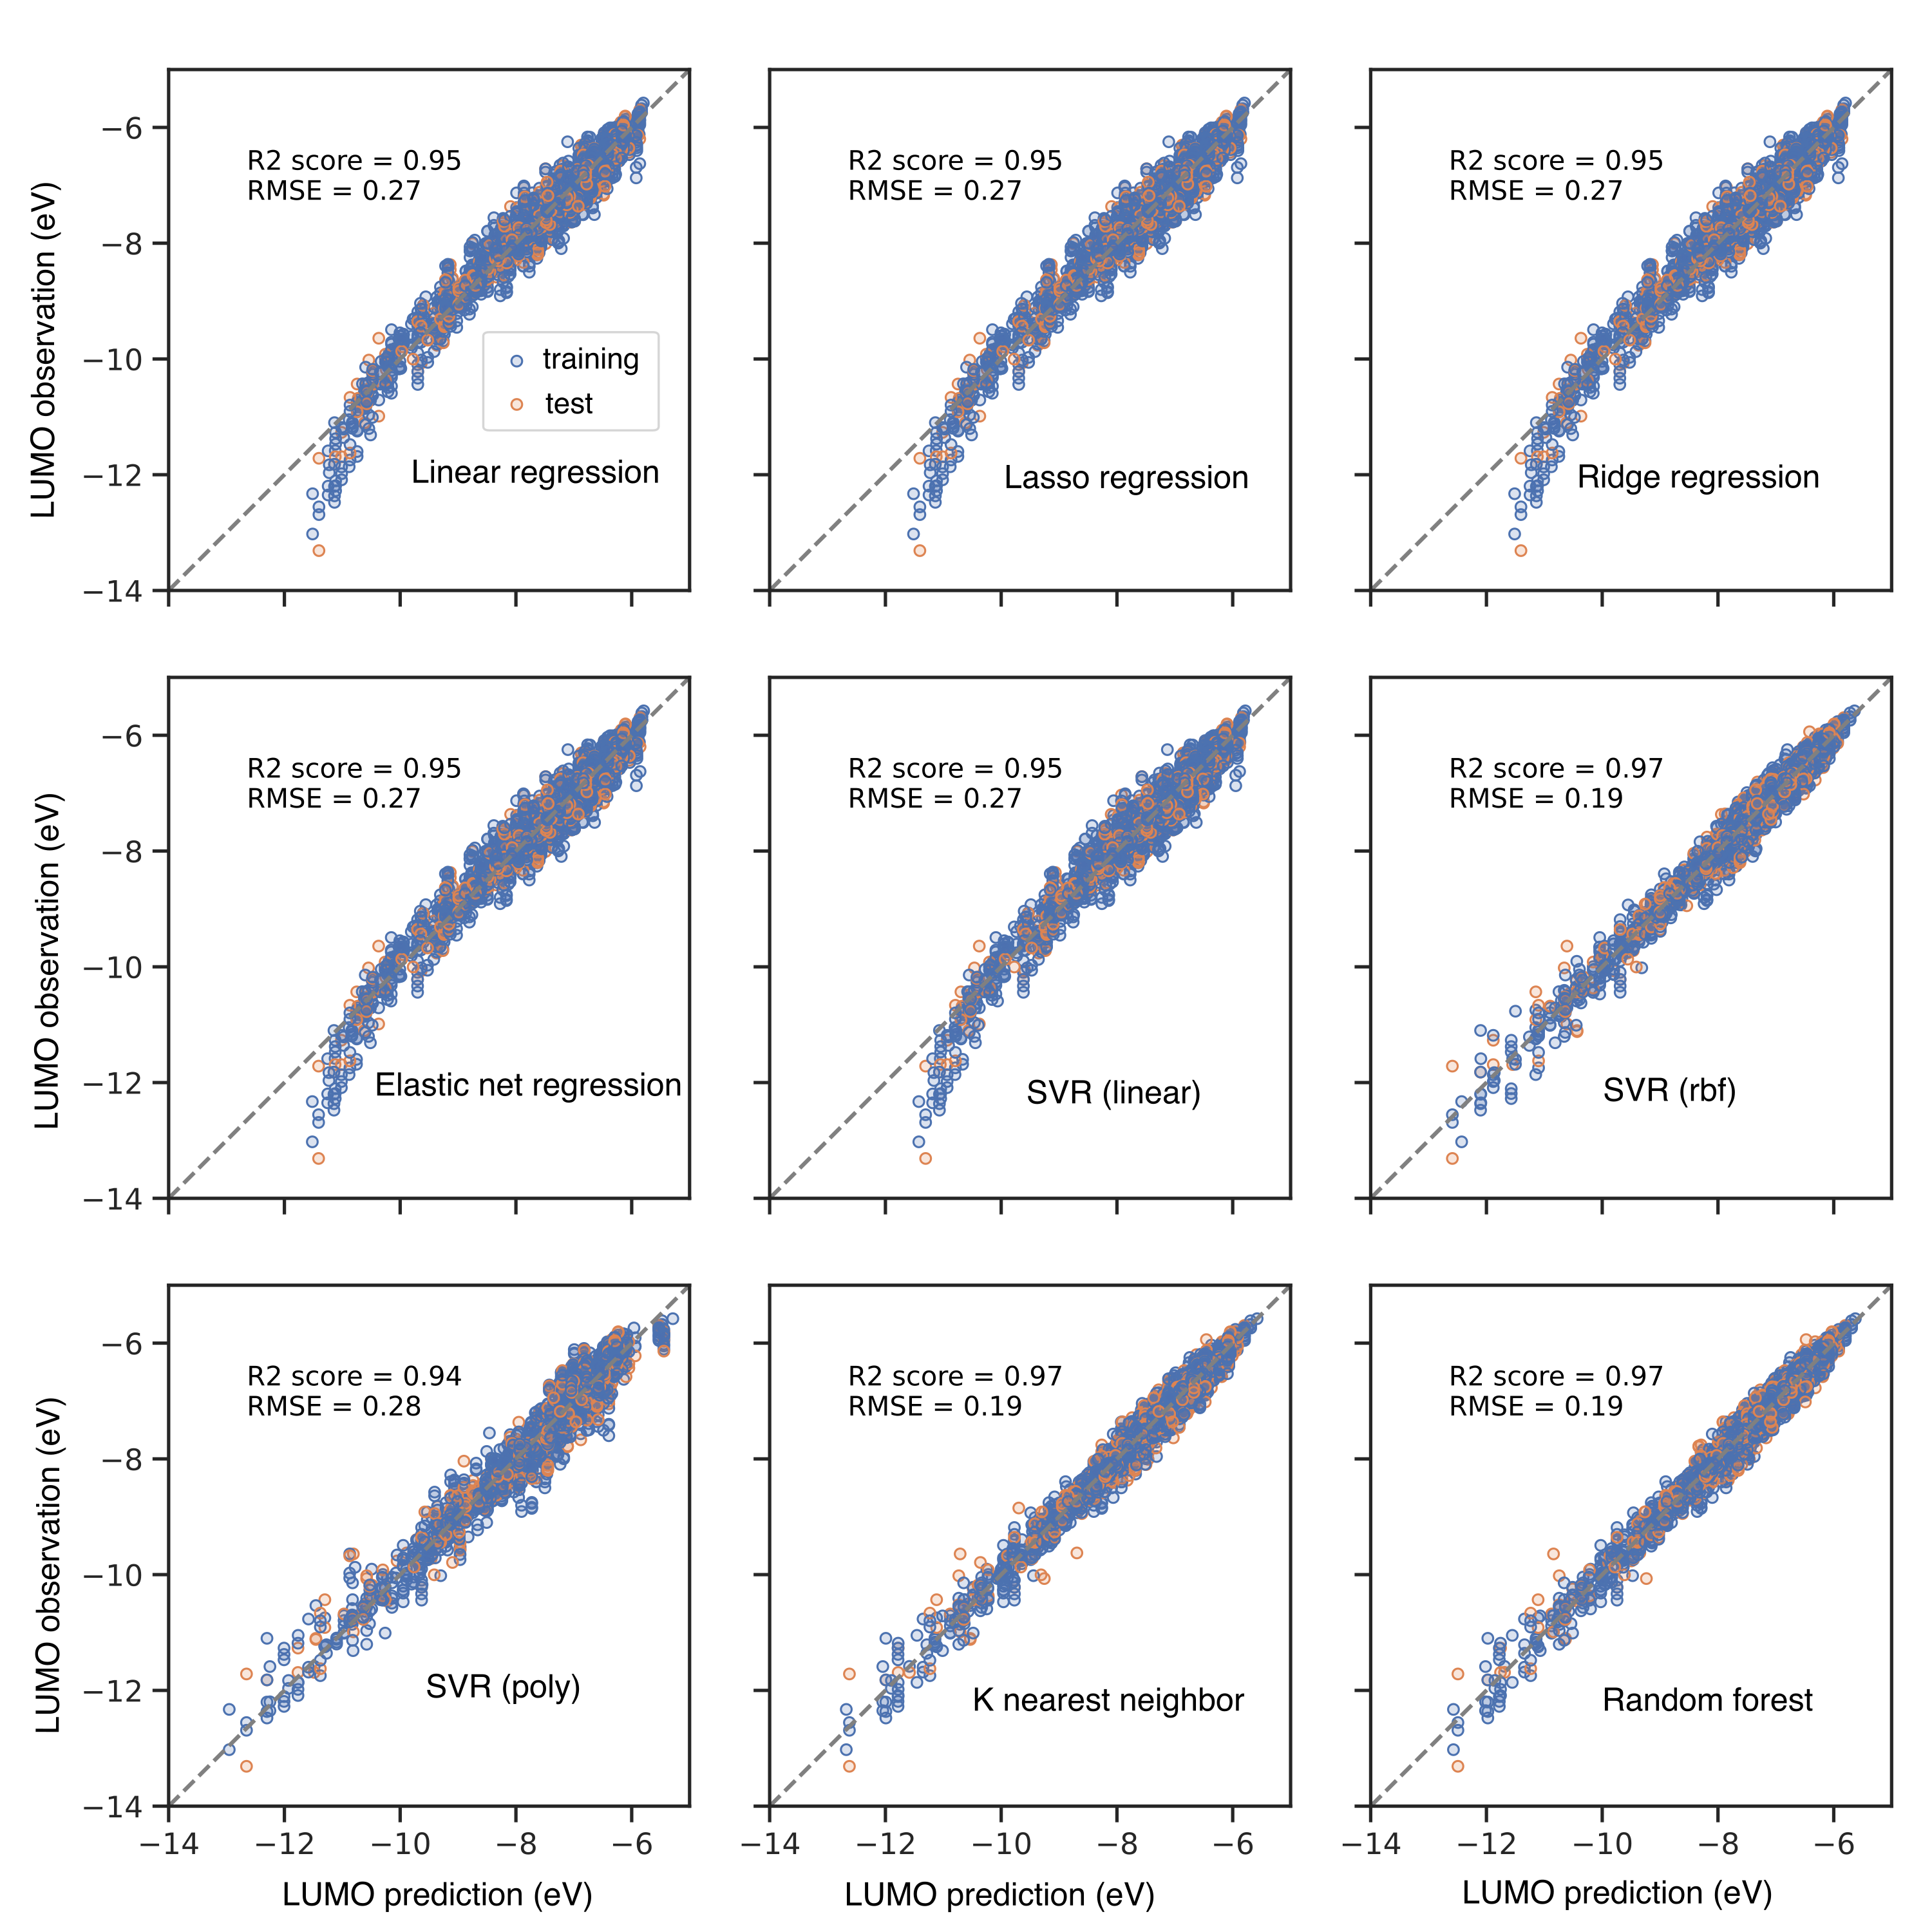
\includegraphics[width=\textwidth]{figures/HT-ML/figure4-14.png}
    \caption{Predicted vs. true values for LUMO level across various ML models.}
    \label{fig:figure4.14}
\end{figure}

\section{Interpretation of structure-property relationships}\label{section:section4-4}

In this section, we explore various approaches to interpreting the machine learning model. We demonstrate how different model interpretation methods can yield slightly different feature importance rankings while still preserving the same underlying physical meaning.

\subsection{Feature coefficient}

In many traditional machine learning approaches—especially linear models—the model parameters (often referred to as coefficients or weights) provide a direct way to interpret how each input feature influences the predicted outcome. In our case, these coefficients offer insight into how various organic descriptors (encoded in the 12-digit fingerprint) affect the HOMO/LUMO energy levels of the organic spacers.

Since our data undergo feature normalization (standardization) before training, two types of coefficients are relevant: normalized feature coefficient (directly reported by the trained model), and unnormalized feature coefficient (raw coefficient rescaled to the original units).

\textbf{Normalized feature coefficient}

During model training, each descriptor is standardized by subtracting its mean and dividing by its standard deviation. As a result, the coefficients reported by the model reflect the effect of a one-standard-deviation change in a descriptor on the predicted HOMO or LUMO. Larger absolute coefficients indicate greater importance, while the sign (positive/negative) denotes whether the feature increases or decreases the predicted value.

\begin{figure}[htbp]
    \centering
    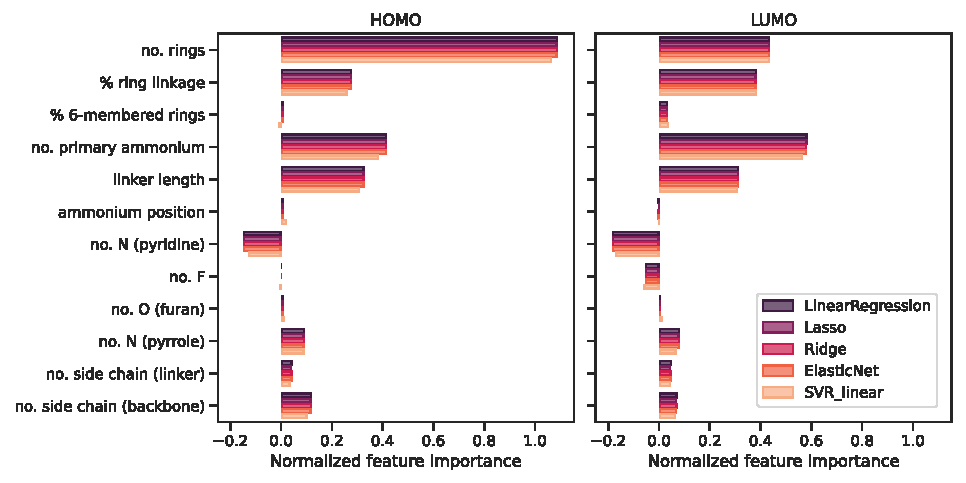
\includegraphics[width=\textwidth]{figures/HT-ML/figure4-15.pdf}
    \caption{Normalized feature coefficients of linear ML models used in this work.}
    \label{fig:figure4.15}
\end{figure}

Figure \ref{fig:figure4.15} compares the normalized feature coefficients from various linear models—including Linear Regression, LASSO, Ridge, Elastic Net, and Linear SVR. All models yield similar coefficients, suggesting that regularization (L1, L2, or a combination) does not drastically alter the identification of the most influential features. Moreover, the consistency in coefficients across models indicates minimal overfitting.

In general, features related to the conjugated backbone (e.g., no. rings) and tethering ammonium groups (e.g., no. primary ammonium) strongly influence both HOMO and LUMO predictions. Notably, most features affect HOMO and LUMO in a comparable manner, implying that variations in the HOMO–LUMO gap primarily arise from a few key descriptors. For HOMO, all features except “no. pyridine-type nitrogens” contribute positively, with number of rings exerting the largest effect. For LUMO, pyridine-type nitrogen and fluorine substitution exert negative contributions, whereas number of rings plays a slightly smaller role compared to HOMO.

Given its L1 regularization, LASSO provides a convenient means of highlighting key features by favouring sparse solutions. Therefore, LASSO regression serves as our representative linear model for subsequent interpretation and prediction, although the insights remain applicable to all linear models.

\textbf{Unnormalized feature coefficient}

While normalized coefficients gauge the effect of a one-standard-deviation change, the unnormalized coefficients express how a one-unit increase in each descriptor affects the HOMO or LUMO in real (eV) units. Consequently, unnormalized coefficients are often more intuitive in a materials science context, where absolute energy shifts matter.

As an example, the LASSO-based HOMO predictor can be written as:

\begin{equation}
\begin{split}
    HOMO &= 1.33\,x_1 + 0.61\,x_2 + 0.05\,x_3 + 1.33\,x_4 + 0.52\,x_5 + 0.18\,x_6 - 0.30\,x_7 + 0.00\,x_8 \\
         &\quad + 0.06\,x_9 + 0.44\,x_{10} + 0.11\,x_{11} + 0.24\,x_{12} - 19.25
\end{split}
\end{equation}


Here, $x_1…x_{12}$ represent the 12 molecular descriptors, and the coefficients specify how changes in each descriptor shift the predicted HOMO (in eV). Notably, $x_1$ and $x_4$—which corresponded to no. rings and no. primary ammonium groups—dominate, indicating their strong contribution to the HOMO level.

\begin{figure}[htbp]
    \centering
    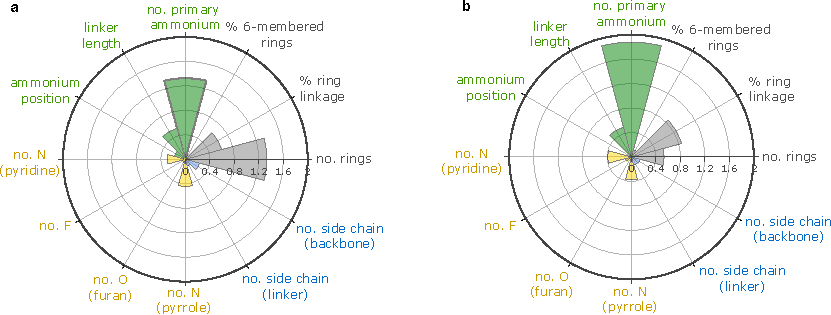
\includegraphics[width=\textwidth]{figures/HT-ML/figure4-16.pdf}
    \caption{Unnormalized feature coefficients (absolute value) from Lasso regression model. }
    \label{fig:figure4.16}
\end{figure}

A similar expression applies to LUMO, and Figure \ref{fig:figure4.16} visualizes the absolute values of the unnormalized coefficient for both HOMO and LUMO in radar plot. Overall, normalized and unnormalized coefficients are consistent; however, descriptors with broader numerical ranges (e.g., number of rings, which varies from 1 to 4) show relatively smaller unnormalized coefficients, whereas features with narrow ranges (e.g., number of primary ammonium groups, which varies from 1 to 2) appear more prominent.

Despite these differences, the physical insights remain the same: conjugation (number of rings) and tethering ammonium groups play crucial roles in frontier orbital energies. The next subsection delves into a comprehensive interpretation of how each feature influences HOMO/LUMO levels.

\subsection{SHAP value analysis}

SHAP (SHapley Additive exPlanations) is a popular method for explaining the output of complex machine learning models. At its core, SHAP leverages concepts from cooperative game theory—specifically Shapley values—to attribute the contribution of each feature to a model’s prediction. To further interpret how individual features influence predictions, we employ SHAP analysis, which assigns each descriptor a contribution (positive or negative) to the final HOMO or LUMO prediction. 

Instead of using the average predicted value (the default SHAP baseline), we use the predicted value of $G_0$ molecule, PDMA, as reference molecule. This makes the SHAP values more physically meaningful because each feature’s contribution is interpreted relative to the G0 molecule rather than to a broad average. Concretely, for each data sample, our model produces 12 SHAP values (one per feature). Summing all 12 SHAP values plus the baseline prediction (the prediction for $G_0$) typically yields the model’s actual prediction for that sample.

\textbf{Global feature importance}

\begin{figure}[htbp]
    \centering
    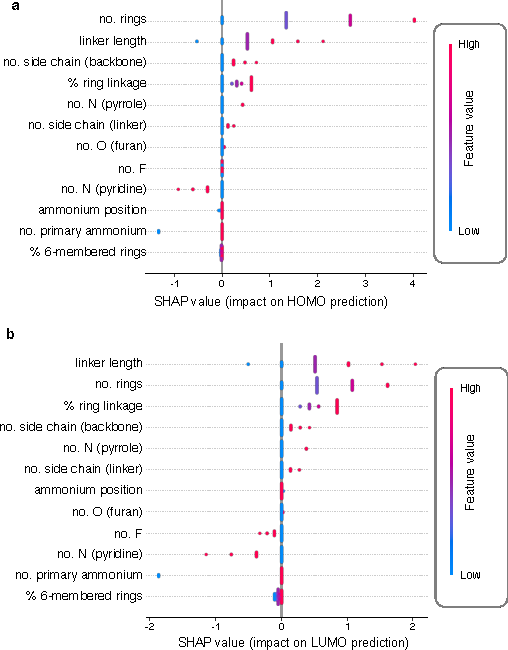
\includegraphics[width=0.8\textwidth]{figures/HT-ML/figure4-17.pdf}
    \caption{SHAP value analysis of HOMO and LUMO predictor.}
    \label{fig:figure4.17}
\end{figure}

Figure \ref{fig:figure4.17} shows a SHAP summary plot (i.e., beeswarm plot), which provides a global view of feature importance and how each feature’s impact varies across samples. The 12 features appear on the y-axis in order of their overall influence, with the most impactful features at the top. Each dot in a row represents a SHAP value for one data point, and the x-axis indicates the magnitude and direction of the feature’s contribution (left for a negative shift from $G_0$, right for a positive shift). Because most features (e.g., no. rings) take discrete values, their SHAP values often cluster in distinct groups rather than forming a continuous distribution. A wider spread of SHAP values in a feature’s row means that feature has a more variable effect across different molecules. For example, “number of rings” can shift the predicted HOMO by as much as 4 eV relative to $G_0$.

The summary plot highlights the influence of key features. Consistent with our analysis of feature coefficient in previous subsection, the features related to the conjugated backbone and tethering ammonium groups being the most significant. Among these, the number of aromatic rings in the conjugated backbone emerges as a critical factor, directly influencing the degree of conjugation—a well-established design rule in organic semiconductors\cite{RN282} that has also found application in 2D perovskites\cite{RN18,RN20}. In addition to conjugation, the analysis underscores the significance of electron richness, another foundational principle in the design of organic semiconductors\cite{RN282}. For tethering ammonium groups, the electron-rich alkyl groups associated with primary ammonium can raise the frontier levels by increasing the linker length or the number of primary ammonium groups. The effect of heteroatom substitution varies depending on the electronic nature of the substituent. For example, pyridine-type nitrogen, being electron-withdrawing, lowers both HOMO and LUMO, while pyrrole-type nitrogen, being electron-donating, raises both levels. Interestingly, fluorination—widely used to enhance stability in 2D perovskite spacers due to the large dipole moment induced by its electron-withdrawing ability\cite{RN84,RN392}—showed a relatively minor influence on the frontier levels in this study. This limited effect may stem from fluorine substitution not directly participating in the conjugated $\pi$-system. While highly electronegative, fluorine’s influence remains localized, resulting in minimal perturbation to the frontier orbitals. 

Compared to feature coefficient discussed in previous section, the linker length emerges as the most influential factor in LUMO prediction. This is because all the data is calibrated by baseline value of $G_0$ molecules, instead of the mean value. This shows that change in linker length can produce the largest deviation from LUMO of $G_0$ molecule.

\textbf{Individual feature importance of representative molecule}

After examining the global summary, we now present visualizations of SHAP values for individual samples. This is achieved using waterfall plots, which decompose a single prediction into its component feature contributions, illustrating how each feature influences the model’s output above or below the baseline (which, in this case, is the $G_0$ molecule). Two categories of organic spacers are analyzed below, molecules with relatively high HOMO, and molecules with relatively low LUMO.

\begin{figure}[htbp]
    \centering
    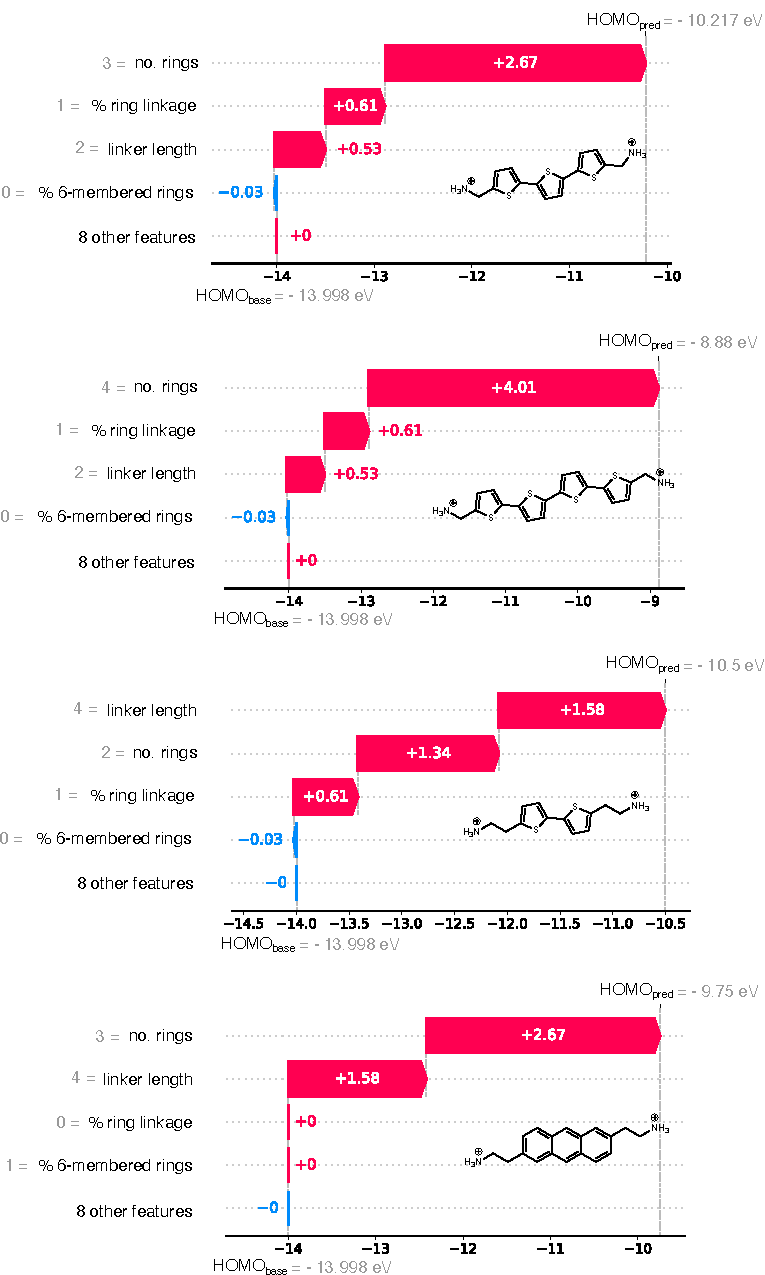
\includegraphics[width=0.8\textwidth]{figures/HT-ML/figure4-18.pdf}
    \caption{SHAP value analysis of representative organic spacers in type IIa.}
    \label{fig:figure4.18}
\end{figure}

Figure \ref{fig:figure4.18} presents SHAP value analysis for four organic spacers with relatively high HOMO levels, which are later validated to achieve Type IIa alignment. The SHAP values are calibrated using the $G_0$ molecule as a baseline (horizontal axis on the left, where HOMO = -13.998 eV). Each feature’s SHAP value is represented by a bar extending to the right (positive contribution, colored in pink) or to the left (negative contribution, colored in blue). The bars are arranged in order of their magnitude of impact, allowing for a visual step-by-step decomposition from the baseline to the final predicted value.

The primary driving factors for a higher HOMO level vary across molecules. For instance, in the first molecule, the most significant contributor is the number of rings, followed by the percentage of ring linkage. In the third molecule, the linker length is the dominant feature, followed by the number of rings.
    
\begin{figure}[htbp]
    \centering
    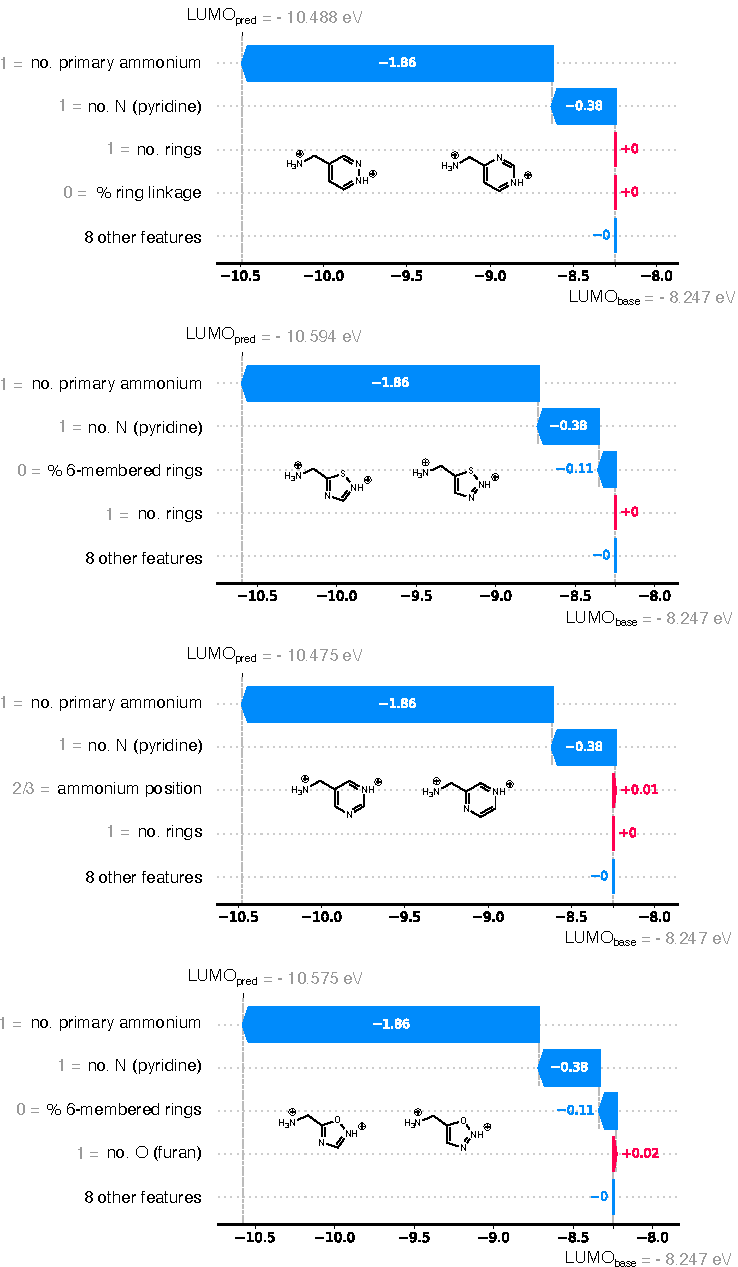
\includegraphics[width=0.8\textwidth]{figures/HT-ML/figure4-19.pdf}
    \caption{SHAP value analysis of representative organic spacers in type IIb.}
    \label{fig:figure4.19}
\end{figure}

Figure \ref{fig:figure4.19} illustrates the SHAP analysis of eight organic spacers predicted to achieve Type IIb alignment, characterized by relatively low LUMO levels.

The results indicate that the most significant factor driving a lower LUMO level across these molecules is the reduction in the number of primary ammonium groups.

These findings demonstrate the predictive capability of the interpretable machine learning model, which allows for the estimation of organic frontier energy levels—and by extension, the energy level alignment of DJ perovskites—for any organic spacer given its fingerprint representation. This capability accelerates the discovery process by enabling the rapid identification of promising candidates with targeted energy level alignment types.

\section{Chapter summary}

This chapter presented a combined high-throughput DFT and machine learning workflow for exploring the chemical space of organic spacers in 2D perovskites. We first generated a diverse library of hypothetical organic cations through systematic morphing operations. High-throughput DFT calculations were then performed to evaluate key physical properties across this expanded chemical space. Machine learning models were trained and benchmarked, achieving high predictive accuracy. Importantly, these models enabled rapid property prediction for large molecular sets and revealed meaningful structure–property relationships. The outcomes from this chapter establish a robust foundation for the inverse design and screening of novel spacer candidates in the following chapters.


